\chapter{Структура баз знаний ostis-систем: иерархическая система предметных областей и соответствующих им онтологий}
\markboth{Структура баз знаний ostis-систем}{Структура баз знаний ostis-систем}
\chapauthortoc{Голенков В.~В.\\Банцевич К.~А.}
\label{chapter_kb}

\vspace{-7\baselineskip}

\begin{SCn}


	\scntext{аннотация}{Глава посвящена онтологическому подходу к проектированию баз знаний интеллектуальных компьютерных систем нового поколения. Данный подход основан на представлении базы знаний как иерархической структуры взаимосвязанных предметных областей и их онтологий, построенных на базе онтологий верхнего уровня.}
\end{SCn}


\section*{Введение в Главу \ref{chapter_kb}}

Развитие информационных технологий привело к расширению многообразия используемой информации, и в следствии, к необходимости создания \textit{интеллектуальных компьютерных систем}, способных оперировать объемными информационными ресурсами. Важнейшими видами таких ресурсов являются \textit{базы знаний}.

\textit{база знаний} представляет собой систематизированную совокупность \textit{знаний}, хранимую в памяти \textit{интеллектуальной компьютерной системы} и достаточную для обеспечения целенаправленного (целесообразного, адекватного) функционирования (поведения) этой системы как в своей внешней среде, так и в своей внутренней среде (в собственной \textit{базе знаний}).

Важным этапом разработки \textit{баз знаний} \textit{интеллектуальных компьютерных систем} является их структуризация. Структуризация \textit{базы знаний}, то есть выделение в ней различных связанных между собой подструктур, необходима по целому ряду причин (см. \scncite{Davydenko2016a}). В частности, это необходимо для обеспечения их синтаксической совместимости, что подразумевает унификацию формы представления \textit{знаний}.

На сегодняшний день существуют десятки моделей представления \textit{знаний}. Каждая из которых адаптирована для представления \textit{знаний} определенного вида, в то время как при создании \textit{интеллектуальных компьютерных систем} часто возникает необходимость представить различные \textit{виды знаний} в рамках одной \textit{базы знаний}. Однако, в настоящее время ни одна из существующих моделей, взятых в отдельности, не может этого обеспечить. 

В связи с этим возникает необходимость в создании универсальной структурированной модели представления \textit{знаний}, которая позволила бы представлять любые \textit{виды знаний} в унифицированном виде.

На сегодняшний день наиболее эффективным средством структуризации различных областей \textit{знаний} являются \textit{онтологии}. Суть онтологического подхода при проектировании \textit{базы знаний} заключается в рассмотрении структуры \textit{базы знаний} как иерархической системы выделенных \textit{предметных областей} и соответствующих им \textit{онтологий}. Однако, онтологически существует множество способов, которыми можно описать реальный мир таким, каким он есть. Решением данной проблемы является использование при проектировании \textit{баз знаний} \textit{интеллектуальных компьютерных систем} \textit{онтологий верхнего уровня}.

Грамотно построенная \textit{онтология верхнего уровня} позволит обеспечить широкую синтаксическую совместимость между большим количеством \textit{онтологий} для различных предметных областей. Поскольку термины предметно-ориентированных \textit{онтологий} подчинены терминам \textit{онтологии} более высокого уровня (см. \scncite{Sowa1995}). 

На сегодняшний день был предпринят ряд попыток по созданию \textit{онтологии верхного уровня}, которая бы позволила обеспечить широкую синтаксическую совместимость разрабатываемых \textit{баз знаний} \textit{интеллектуальных компьютерных систем}. Однако после анализа существующих \textit{онтологий верхнего уровня}, который подробно представлен в \textit{~\ref{sec_top_level_ontologies}~\nameref{sec_top_level_ontologies}}, был сделан вывод, что попытки создать универсальную \textit{онтологию верхнего уровня}, способную обеспечить совместимость \textit{интеллектуальных компьютерных систем}, не привели к ожидаемым результатам, поскольку имеют ряд ключевых недостатков.

Отсутствие \textit{онтологии верхнего уровня}, которая бы позволила решить проблему проектирования и разработки \textit{баз знаний} \textit{интеллектуальных компьютерных систем}, приводит к несовместимости разрабатываемых \textit{интеллектуальных компьютерных систем}. Исходя из вышесказанного, возникает необходимость в построении такой системы \textit{онтологий верхнего уровня}, которая могла бы обеспечить синтаксическую совместимость между большим количеством \textit{онтологий} различных \textit{предметных областей} \textit{баз знаний} \textit{интеллектуальных компьютерных систем}. 

Для решения представленных проблем необходимо согласовать трактовку таких понятий, как \textit{структура}, \textit{семантическая окрестность}, \textit{предметная область}, \textit{онтология}, поскольку данные понятия являются базовыми классами сущностей, составляющими основу для структуризации \textit{баз знаний} интеллектуальных систем (см. \scncite{Davydenko2017a}). .

Онтологическая модель, построенная на основе данных понятий, станет \textit{Ядром базы знаний}, обеспечивающим совместимость интеллектуальных системы, за счет унифицированного представления знаний (см. \scncite{Bantsevich2022a}). Следует отметить, что в зависимости от специфики разрабатываемых систем их \textit{базы знаний} могут расширяться, однако, онтологическая модель, лежащая в основе \textit{Ядра}, позволит обеспечить дальнейшую совместимость разрабатываемых систем.

\section{Формализация понятия знания и формальные модели баз знаний ostis-систем}
\label{sec_kb}

В рамках модели \textit{баз знаний} ostis-систем выделяются синтаксически корректные (для соответствующего языка) и семантически целостные информационные конструкции. Такие конструкции будем называть \textit{знаниями}.

\begin{SCn}
	\scnheader{знание}
	\scnidtf{синтаксически корректная (для соответствующего языка) и семантически целостная информационная конструкция}
	\scnsubset{информационная конструкция}
	\scnrelfrom{покрытие}{вид знаний}
	\begin{scnindent}
		\scnidtf{Множество \myuline{всевозможных} видов знаний}
	\end{scnindent}
\end{SCn}

Тот факт, что семейство \textit{видов знаний} является покрытием \textit{Множества всевозможных знаний}, означает то, что каждое знание принадлежит по крайней мере одному выделенному нами \textit{виду знаний}.

\begin{SCn}
	\scnheader{вид знаний}
	\scnhaselement{спецификация}
	\begin{scnindent}
		\scnidtf{описание заданной сущности}
		\scnsuperset{спецификация материальной сущности}
		\scnsuperset{спецификация обратной сущности, не являющейся множеством}
		\begin{scnindent}
			\scnsuperset{спецификация геометрической точки}
			\scnsuperset{спецификация числа}
		\end{scnindent}
		\scnsuperset{спецификация множества}
		\begin{scnindent}
			\scnsuperset{спецификация связи}
			\scnsuperset{спецификация структуры}
			\scnsuperset{спецификация класса}
			\begin{scnindent}
				\scnsuperset{спецификация класса сущностей, не являющихся множествами}
				\scnsuperset{спецификация отношения}
				\begin{scnindent}
					\scnidtf{спецификация класса связей (связок)}
				\end{scnindent}
				\scnsuperset{спецификация класса классов}
				\begin{scnindent}
					\scnsuperset{спецификация параметра}
				\end{scnindent}
				\scnsuperset{спецификация класса структур}
				\scnsuperset{спецификация понятий}
					\begin{scnindent}
					\scnsuperset{пояснение}
					\scnsuperset{определение}
					\scnsuperset{утверждение}				
					\end{scnindent}
			\end{scnindent}
		\end{scnindent}
		\scnsuperset{семантическая окрестность}
		\scnsuperset{однозначная спецификация}
		\scnsuperset{сравнительный анализ}
		\scnsuperset{достоинства}
		\scnsuperset{недостатки}
		\scnsuperset{структура специфицируемой сущности}
		\scnsuperset{принципы, лежащие в основе}
		\scnsuperset{обоснование предлагаемого решения}
	\end{scnindent}
	\scnhaselement{сравнение}
	\scnhaselement{высказывание}
		\begin{scnindent}
		\scnsuperset{фактографическое высказывание}
		\scnsuperset{закономерность}
		\end{scnindent}
	\scnhaselement{формальная теория}
	\scnhaselement{предметная область}
	\scnhaselement{предметная область и онтология}
	\scnhaselement{метазнание}
	\begin{scnindent}
		\scnidtf{спецификация знания}
		\scnsuperset{аннотация}
		\scnsuperset{введение}
		\scnsuperset{предисловие}
		\scnsuperset{заключение}
		\scnsuperset{онтология}
		\begin{scnindent}
			\scnsuperset{онтология предметной области}
			\begin{scnindent}
				\scnsuperset{структурная онтология предметной области}
				\scnsuperset{теоретико-множественная онтология предметной области}
				\scnsuperset{логическая онтология предметной области}
				\scnsuperset{терминологическая онтология предметной области}
				\scnsuperset{объединенная онтология предметной области}
			\end{scnindent}
		\end{scnindent}
	\end{scnindent}
	\scnhaselement{задача}
	\scnhaselement{план}
	\scnhaselement{протокол}
	\scnhaselement{результативная часть протокола}
	\scnhaselement{метод}
	\scnhaselement{технология}
	\scnhaselement{база знаний}
\end{SCn}


Даже небольшой перечень \textit{видов знаний} свидетельствует об огромном многообразии \textit{видов знаний}.

\textit{знания} разделяются на \textit{декларативные} и \textit{процедурные}. Под \textit{декларативными знаниями} понимаются \textit{знания}, которые имеют только \textit{денотационную семантику}, которая представляется в виде семантической \textit{спецификации} системы понятий, используемых в этом \textit{знании}. Под \textit{процедурным знанием} понимается \textit{знание}, имеющее не только \textit{денотационную семантику}, но и \textit{операционную семантику}, которая представляется в виде семейства \textit{спецификаций агентов}, осуществляющих интерпретацию \textit{процедурного знания}, направленную на решение некоторой инициированной задачи.

В рамках \textit{Технологии OSTIS} также выделяются \textit{отношения, заданные на множестве знаний}.

\begin{SCn}
	\scnheader{отношение, заданное на множестве знаний}
	\scnhaselement{дочернее знание*}
	\begin{scnindent}
		\scnidtf{знание, которое от "материнского"{} знания наследует все описанные там свойства объектов исследования}
		\scnsuperset{дочерний раздел*}
			\begin{scnindent}
			\scnidtf{частный раздел*}
		\end{scnindent}
		\scnsuperset{дочерняя предметная область и онтология*}
	\end{scnindent}
	\scnhaselement{спецификация*}
	\begin{scnindent}
		\scnidtf{быть знанием, которое является спецификацией (описанием) заданной сущности}
	\end{scnindent}
	\scnhaselement{онтология*}
	\begin{scnindent}
		\scnidtf{быть семантической спецификацией заданного знания*}
	\end{scnindent}
	\scnhaselement{семантическая эквивалентность*}
	\scnhaselement{следовательно*}
	\begin{scnindent}
		\scnidtf{логическое следствие*}
	\end{scnindent}
	\scnhaselement{логическая эквивалентность*}
\end{SCn}

Важным \textit{видом знаний} являются \textit{базы знаний}.

\begin{SCn}
\scnheader{база знаний}
\scnidtf{совокупность знаний, хранимых в памяти интеллектуальной компьютерной системы и \myuline{достаточных} для того, чтобы указанная система удовлетворяла соответствующим предъявляемым к ней требованиям (в частности, чтобы она имела соответствующий уровень интеллекта)}
\scnidtf{систематизированная совокупность знаний, хранимая в памяти интеллектуальной компьютерной системы и достаточная для обеспечения целенаправленного (целесообразного, адекватного) функционирования (поведения) этой системы как в своей внешней среде, так и в своей внутренней среде (в собственной базе знаний)}
\end{SCn}

\begin{comment}
	
Представленным понятиям соответствует \textit{Предметная область знаний и баз знаний ostis-систем}, в которой они подробно рассматриваются. 
 
\begin{SCn}
	\scnheader{Предметная область знаний и баз знаний ostis-систем}
	\scniselement{предметная область}
	\scnhaselementrole{максимальный класс объектов исследования}{знание}
	\begin{scnhaselementrolelist}{исследуемый класс классов}
		\scnitem{вид знаний}
		\scnitem{отношение, заданное на множестве знаний}
	\end{scnhaselementrolelist}
\end{SCn}

Важно отметить, что одним из основных факторов, определяющими качество \textit{интеллектуальной компьютерной системы}, является качественная структуризация (систематизация) и \myuline{стратификация} \textit{базы знаний} \textit{интеллектуальной компьютерной системы}.
	

\section{Формализация понятия структуры}
\label{sec_structure}

\begin{SCn}
	\begin{scnrelfromlist}{ключевое понятие}
		\scnitem{структура}
	\end{scnrelfromlist}
\end{SCn}

\begin{SCn}
	\begin{scnrelfromlist}{ключевое знание}
		\scnitem{Классификация структур}
	\end{scnrelfromlist}
\end{SCn}

\begin{SCn}
	\begin{scnrelfromlist}{ключевой знак}
		\scnitem{Предметная область структур}
	\end{scnrelfromlist}
\end{SCn}

Существующие подходы к разработке \textit{баз знаний} основываются на рассмотрении в качестве объектов спецификации конкретных элементов \textit{базы знаний} (классов, экземпляров, отношений и так далее). Однако при накоплении больших объемов информации в \textit{базе знаний} возникает необходимость выделять целые фрагменты \textit{базы знаний} и иметь возможность их специфицировать, рассматривая как отдельные сущности. 

Такой фрагмент базы знаний назван \textit{структурой (sc-структурой)}. Под \textit{структурой} будем понимать множество \textit{sc-элементов}, удаление одного из которых может привести к нарушению целостности этого множества. Каждая \textit{структура} представляет собой \textit{sc-элемент}, обозначающий некоторый текст \textit{SC-кода}, который может быть объектом спецификации, в том числе входить в состав других \textit{структур}, быть связанным с другими сущностями различными отношениями. 

Понятие \textit{структуры} является основой для представления \textit{знаний}, \textit{метазнаний} и их структуризации, а также является одним из наиболее общих (с точки зрения уточнения семантики) понятий при описании свойств какого-либо объекта. 

\textit{структура} может изображаться путем явного указания всех пар принадлежности элементов этой \textit{структуре}, а также в виде контура, содержащего все элементы, входящие в состав этой \textit{структуры}, что продемонстрировано на рисунке \textit{\nameref{fig:structure_example}}.

\begin{figure}[H]
	\caption{SCg-текст. Пример полного и сокращенного представления структуры в SCg-коде}
	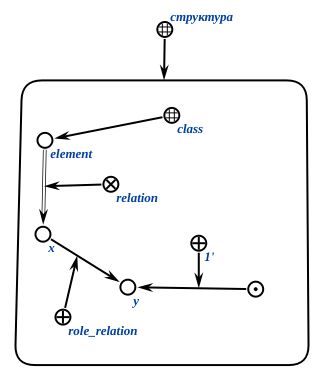
\includegraphics[scale=0.7]{author/part2/figures/chapter_kb/structure.png}
	\label{fig:structure_example}
\end{figure}


Рассмотрим типологию \textit{структур}, описываемых в \textit{базе знаний}.

\textit{структуре}, представленной в \textit{SC-коде}, поставим в соответствие орграф, вершинами которого являются \textit{sc-элементы}, а дугами --- связки отношений инцидентности, связывающие sc-коннекторы с инцидентными им \textit{sc-элементами}, которые являются компонентами указанных sc-коннекторов. Если полученный таким способом орграф является связным орграфом, то исходную структуру будем считать \textit{связной структурой}. Если полученный таким способом орграф не является связным орграфом, то исходную структуру будем считать \textit{несвязной структурой}.

\begin{SCn}
	\scnheader{структура}
	\begin{scnrelfromset}{разбиение}
		\scnitem{связная структура}
		\scnitem{несвязная структура}
	\end{scnrelfromset}
\end{SCn}

Под \textit{тривиальной структурой} понимается \textit{структура}, не содержащая в качестве элементов связок. В свою очередь, под \textit{нетривиальной структурой} понимается \textit{структура}, среди элементов которой есть хотя бы одна связка.

\begin{SCn}
	\scnheader{структура}
	\begin{scnrelfromset}{разбиение}
		\scnitem{тривиальная структура}
		\scnitem{нетривиальная структура}
	\end{scnrelfromset}
\end{SCn}

По признаку стационарности/нестационарности выделяются \textit{динамические структуры} (процессы) --- \textit{структуры}, состав которых меняется с течением времени, и \textit{статические структуры} --- \textit{структуры}, состав которых не меняется с течением времени.

\begin{SCn}
	\scnheader{структура}
	\begin{scnrelfromset}{разбиение}
		\scnitem{процесс}
		\begin{scnindent}
			\scnidtf{динамическая структура}
			\scnidtf{нестационарная структура}
		\end{scnindent}
		\scnitem{статическая структура}
		\begin{scnindent}
			\scnidtf{стационарная структура}
			\scnidtf{структура, не изменяющаяся во времени}
		\end{scnindent}
	\end{scnrelfromset}
\end{SCn}

По признаку времени существования выделяются \textit{временные структуры} и \textit{постоянно существующие структуры}.

\begin{SCn}
	\scnheader{структура}
	\begin{scnrelfromset}{разбиение}
		\scnitem{временная структура}
		\begin{scnindent}
			\scnidtf{(структура $\cap$ временная сущность)}
		\end{scnindent}
		\scnitem{постоянно существующая структура}
		\begin{scnindent}
			\scnidtf{(структура $\cap$ постоянная сущность)}
		\end{scnindent}
	\end{scnrelfromset}
\end{SCn}

\begin{comment}
	
В рамках заданной \textit{структуры} ее элементы можно классифицировать по заданным признакам:\\

\begin{SCn}
\begin{scnitemize}
	\item насколько полно в рамках \myuline{заданной \textit{структуры}} представлено множество, обозначаемое \textit{заданным sc-элементом} вместе с соответствующими дугами принадлежности;
	\item существуют ли в рамках \uline{заданной \textit{структуры}} \textit{sc-элементы}, обозначающие множества, являющиеся надмножествами того множества, которое обозначается \uline{заданным \textit{sc-элементом}};
	\item уровень («этаж») иерархии перехода от знаков к метазнакам для \myuline{заданного \textit{sc-элемента}} в рамках заданной \textit{структуры}.
\end{scnitemize}
\end{SCn}

\bigskip
Для формального представления \textit{структур} используются понятия, описывающие роли элементов в рамках структуры. \textbf{\textit{элемент структуры\scnrolesign}} --- \textit{неосновное понятие}, \textit{ролевое отношение}, указывающее на все элементы каждой \textit{структуры}. Пример описания элементов структуры представлен на рисунке \textit{\nameref{fig:structure_elements}}.

\begin{SCn}
	\scnheader{элемент структуры\scnrolesign}
	\begin{scnrelfromset}{разбиение}
		\scnitem{непредставленное множество\scnrolesign}
		\begin{scnindent}
			\scnidtf{множество, не представленное в рамках данной структуры\scnrolesign}
		\end{scnindent}
		\scnitem{полностью представленное множество\scnrolesign}
		\begin{scnindent}
			\scnidtf{множество, полностью представленное в рамках данной структуры\scnrolesign}
		\end{scnindent}
		\scnitem{частично представленное множество\scnrolesign}
		\begin{scnindent}
			\scnidtf{множество, частично представленное в рамках данной структуры\scnrolesign}
		\end{scnindent}
		\scnitem{элемент структуры, не являющийся множеством\scnrolesign}
	\end{scnrelfromset}
\begin{scnrelfromset}{разбиение}
	\scnitem{максимальное множество\scnrolesign}
	\scnitem{немаксимальное множество\scnrolesign}
\end{scnrelfromset}

\scnheader{максимальное множество\scnrolesign}
\scnexplanation{\textbf{\textit{максимальное множество\scnrolesign}} --- \textit{ролевое отношение}, связывающее \textit{структуру} со знаком множества, для которого не существует множества, которое было бы надмножеством указанного множества и знак которого был бы элементом этой же структуры.}

\scnheader{немаксимальное множество\scnrolesign}
\scnexplanation{\textbf{\textit{немаксимальное множество\scnrolesign}} --- \textit{ролевое отношение}, связывающее \textit{структуру} со знаком множества, для которого в рамках данной \textit{структуры} существует множество, являющееся надмножеством указанного множества.}

\scnheader{первичный элемент\scnrolesign}
\scnidtf{первичный элемент данной структуры\scnrolesign}
\scnidtf{sc-элемент первого уровня в рамках данной структуры\scnrolesign}
\scniselement{ролевое отношение}
\scnsubset{элемент структуры\scnrolesign}
\scnexplanation{\textbf{\textit{первичный элемент\scnrolesign}} --- ролевое отношение, указывающее на элемент \textit{структуры}, являющийся либо терминальным элементом, либо знаком множества, такого что не существует другого элемента этой же структуры, который был бы элементом множества, обозначаемого первым из указанных элементов структуры. При этом соответствующая пара принадлежности может существовать, но в состав данной структуры не входить.}

\scnheader{вторичный элемент\scnrolesign}
\scnidtf{вторичный элемент данной структуры\scnrolesign}
\scnidtf{элемент данной структуры имеющий семантический уровень более 2\scnrolesign}
\scnidtf{непервичный элемент\scnrolesign}
\scniselement{ролевое отношение}
\scnsubset{элемент структуры\scnrolesign}
\scnexplanation{\textbf{\textit{вторичный элемент\scnrolesign}} --- ролевое отношение, указывающее на элемент структуры, обозначающий множество, все или некоторые элементы которого являются элементами указанной структуры.}
\scnsuperset{элемент второго уровня\scnrolesign}

\scnheader{элемент второго уровня\scnrolesign}
\scniselement{ролевое отношение}
\scnexplanation{\textbf{\textit{элементом второго уровня\scnrolesign}} в рамках заданной \textit{структуры} может быть связка первичных элементов, тривиальная структура из первичных элементов или класс первичных элементов.}

\scnheader{структура второго уровня\scnrolesign}
\scnexplanation{\textbf{\textit{структура второго уровня}} --- \textit{структура}, среди элементов которой есть хотя бы один \textit{элемент второго уровня\scnrolesign}.}
\end{SCn}

\begin{figure}[H]
	\caption{SCg-текст. Пример описания элементов структуры на SCg-коде}
	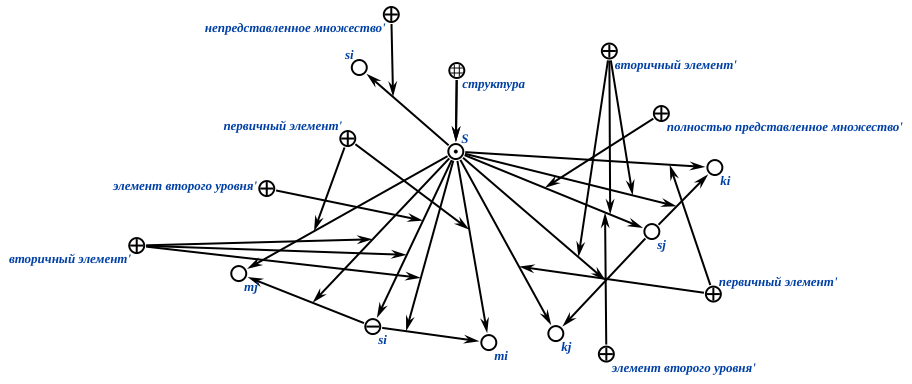
\includegraphics[scale=0.7]{author/part2/figures/chapter_kb/structure_elements.png}
	\label{fig:structure_elements}
\end{figure}

Тот факт, что в качестве формальной основы представления \textit{знаний} в \textit{SC-коде} лежит теория графов и теория множеств, позволяет анализировать не
только внешние связи рассматриваемого фрагмента \textit{базы знаний} с другими
элементами \textit{базы знаний}, но и внутреннюю структуру этих фрагментов с необходимой степенью детализации, то есть выявлять в \textit{базе знаний} аналогии, сходства, различия, строить различные виды соответствий между фрагментами.

Между \textit{структурами} можно определять ряд соответствий, таких как \textit{гомоморфизм}, \textit{полиморфизм}, \textit{автоморфизм}, \textit{изоморфизм}, а также \textit{аналогичность структур}, что позволяет фиксировать факт наличия некоторой аналогии, сходства и различия некоторых подструктур рассматриваемых \textit{структур}.
	
\begin{SCn}
	
\scnheader{полиморфность*}
\scnsubset{соответствие*}
\scniselement{бинарное отношение}
\scnexplanation{\textbf{\textit{полиморфность*}} --- это \textit{соответствие}, заданное на \textit{структурах}, при котором каждому элементу из области определения соответствия (первой \textit{структуры}) ставится в соответствие один или более элемент из области значения соответствия (второй \textit{структуры}), при этом существует хотя бы один элемент области определения соответствия, которому соответствуют два или более элемента из области значения соответствия.}

\scnheader{полиморфизм*}
\scniselement{бинарное отношение}

\scnheader{гомоморфность*}
\scnidtf{гомоморфность структур*}
\scnsubset{соответствие*}
\scniselement{бинарное отношение}
\scnexplanation{\textbf{\textit{гомоморфность*}} --- это \textit{соответствие}, заданное на \textit{структурах}, при котором каждому элементу из области определения соответствия (первой \textit{структуры}) ставится в соответствие только один элемент из области значения соответствия (второй \textit{структуры}).}


\scnheader{гомоморфизм*}
\scniselement{бинарное отношение}

\scnheader{изоморфность*}
\scnidtf{изоморфное соответствие*}
\scnidtf{изоморфность структур*}
\scnsubset{гомоморфность*}
\scniselement{бинарное отношение}
\scnexplanation{\textbf{\textit{изоморфность*}} --- это \textit{гомоморфность*}, при которой для каждого элемента из области значения существует ровно один соответствующий элемент из области определения.}

\scnheader{изоморфизм*}
\scniselement{бинарное отношение}

\scnheader{автомоморфность*}
\scnsubset{гомоморфность*}
\scniselement{бинарное отношение}
\scnexplanation{\textbf{\textit{автоморфность*}} --- это \textit{изоморфность*}, у которой область определения соответствия и область значения соответствия совпадают.}

\scnheader{автоморфизм*}
\scniselement{бинарное отношение}
\end{SCn}

\bigskip
Отдельное внимание стоит уделить соответствию \textit{аналогичность структур}, которое фиксирует факт наличия некоторой аналогии на подструктурах (подмножествах) указанных \textit{структур}. Каждой ориентированной паре, принадлежащей \textit{аналогичности структур}, может быть поставлено в соответствие множество пар, задающих \textit{сходства} некоторых подструктур и \textit{различия} некоторых подструктур исходных структур. Пример данного отношения представлен на рисунке \textit{\nameref{fig:analogy_of_structures}}.


\begin{SCn}
\scnheader{аналогичность структур*}
\scnsubset{соответствие*}
\scniselement{бинарное отношение}
\scnexplanation{\textbf{\textit{аналогичность структур*}} --- \textit{соответствие*}, задаваемое на структурах, и фиксирующее факт наличия некоторой аналогии на подструктурах (подмножествах) указанных структур. Каждой ориентированной паре, принадлежащей \textbf{\textit{аналогичности структур*}} может быть поставлено в соответствие множество пар, задающих \textit{сходства*} некоторых подструктур и \textit{различия*} некоторых подструктур исходных структур.}


\scnheader{сходство*}
\scniselement{бинарное отношение}

\scnheader{различие*}
\scniselement{бинарное отношение}	
\end{SCn}

\begin{figure}[H]
	\caption{SCg-текст. Пример отношения аналогичности структур}
	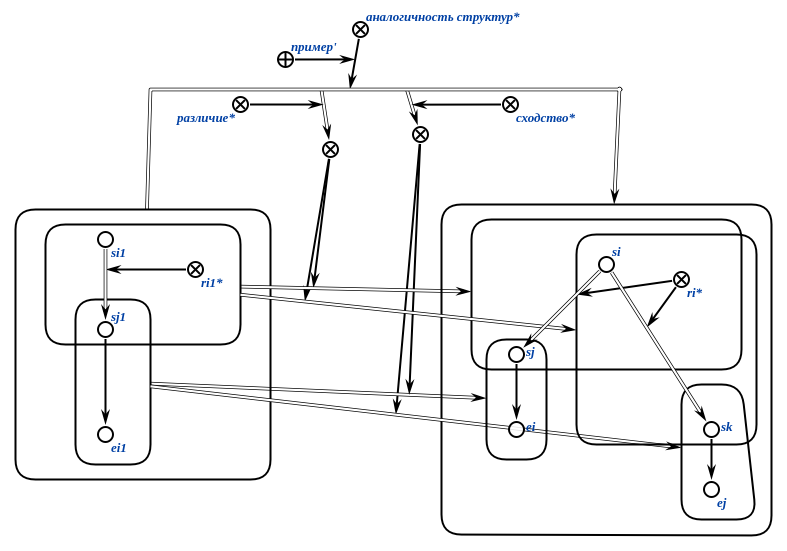
\includegraphics[scale=0.7]{author/part2/figures/chapter_kb/analogy.png}
	\label{fig:analogy_of_structures}
\end{figure}

Соответствия на \textit{структурах} являются частным случаем \textit{метазнаний}. Используя такие соответствия, можно описывать в \textit{базе знаний} и анализировать в дальнейшем, например, сходства и отличия различных фрагментов \textit{базы знаний}, в том числе различных \textit{предметных областей}.

Понятие \textit{структуры} подробно рассматривается в \textit{Предметной области структур}.

\begin{SCn}
	\scnheader{Предметная область структур}
	\scniselement{предметная область}
	\scnhaselementrole{максимальный класс объектов исследования}{структура}
	\begin{scnhaselementrolelist}{класс объектов исследования}
		\scnitem{связная структура}
		\scnitem{несвязная структура}
		\scnitem{тривиальная структура}
		\scnitem{нетривиальная структура}
	\end{scnhaselementrolelist}
	\begin{scnhaselementrolelist}{исследуемое отношение}
		\scnitem{элемент структуры\scnrolesign}
		\scnitem{непредставленное множество\scnrolesign}
		\scnitem{полностью представленное множество\scnrolesign}
		\scnitem{частично представленное множество\scnrolesign}
		\scnitem{элемент структуры, не являющийся множеством\scnrolesign}
		\scnitem{максимальное множество\scnrolesign}
		\scnitem{немаксимальное множество\scnrolesign}
		\scnitem{первичный элемент\scnrolesign}
		\scnitem{вторичный элемент\scnrolesign}
		\scnitem{элемент второго уровня\scnrolesign}
		\scnitem{метасвязь\scnrolesign}
		\scnitem{полиморфность*}
		\scnitem{полиморфизм*}
		\scnitem{гомоморфность*}
		\scnitem{гомоморфизм*}
		\scnitem{изоморфность*}
		\scnitem{изоморфизм*}
		\scnitem{автоморфность*}
		\scnitem{автоморфизм*}
		\scnitem{аналогичность структур*}
		\scnitem{сходство*}
		\scnitem{различие*}
	\end{scnhaselementrolelist}
\end{SCn}
\end{comment}

\section{Формализация понятия семантической окрестности}
\label{sec_sem_neighborhood}

Для спецификации отдельных сущностей в рамках \textit{базы знаний} вводится понятие \textit{семантической окрестности}. 

\textit{семантическая окрестность} представляет собой спецификацию заданной сущности, знак которой указывается как ключевой элемент этой спецификации. В отличие от других \textit{видов знаний}, \textit{семантическая окрестность} имеет только один ключевой элемент.

Набор признаков, по которым можно специфицировать сущности, различен. Кроме того, может возникнуть необходимость специфицировать одну и ту же сущность в различных аспектах и явно фиксировать эти аспекты в \textit{базе знаний}.

Так, например, одну и ту же персону можно описывать с профессиональной, медицинской, гражданской и других точек зрения, как представлено на рисунке \textit{\nameref{fig:semantic_neighborhood}}. 

\begin{figure}[H]
	\caption{SCg-текст. Пример описания семантических окрестностей в SC-коде}
	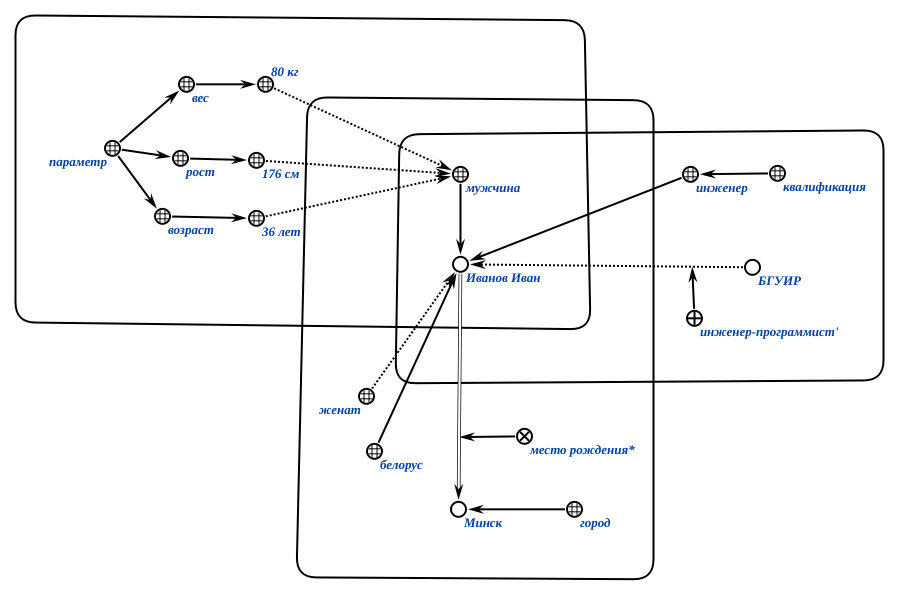
\includegraphics[scale=0.7]{author/part2/figures/chapter_kb/semantic_neighborhood.png}
	\label{fig:semantic_neighborhood}
\end{figure}

Понятие \textit{семантической окрестности}, как и любой другой \myuline{семантически} выделяемый класс \textit{знаний}, абсолютно не зависит от \textit{языка представления знаний}. Этим \textit{языком} может быть не только \textit{SC-код} или другой \textit{формальный язык представления знаний} или даже \textit{естественный язык}, тексты которых в \textit{памяти ostis-системы} представляются в виде \textit{файлов}.

Возможность описания различных свойств одного и того же объекта достигается за счет выделения различных классов \textit{семантических окрестностей} и выделения набора признаков, определяющих тот или иной класс \textit{семантических окрестностей}.

\begin{comment}


Перечислим основные виды \textit{семантических окрестностей}.

\begin{SCn}
\scnheader{семантическая окрестность}
\scnidtf{sc-окрестность}
\scnidtf{семантическая окрестность, представленная в виде sc-текста}
\scnidtf{sc-текст, являющийся семантической окрестностью некоторого sc-элемента}
\scnidtf{спецификация заданной сущности, знак которой указывается как ключевой элемент этой спецификации}
\scnidtf{описание заданной сущности, знак которой указывается как ключевой элемент этой спецификации}
\scnsubset{знание}
\scnsuperset{семантическая окрестность по инцидентным коннекторам}
\scnsuperset{полная семантическая окрестность}
\scnsuperset{базовая семантическая окрестность}
\scnsuperset{специализированная семантическая окрестность}

\scnheader{семантическая окрестность по инцидентным коннекторам}
\scnsuperset{семантическая окрестность по выходящим дугам}
\scnsuperset{семантическая окрестность по входящим дугам}
\scnidtftext{пояснение}{вид \textit{семантической окрестности}, в которую входят все коннекторы, инцидентные заданному элементу, а также все элементы, инцидентные указанным коннекторам.}

\scnheader{семантическая окрестность по выходящим дугам}
\scnsuperset{семантическая окрестность по выходящим дугам принадлежности}
\scnidtftext{пояснение}{вид \textit{семантической окрестности}, в которую входят все дуги, выходящие из заданного sc-элемента и вторые компоненты этих дуг. Также указывается факт принадлежности этих дуг каким-либо отношениям.}

\scnheader{семантическая окрестность по выходящим дугам принадлежности}
\scnidtftext{пояснение}{вид \textit{семантической окрестности}, в которую входят все дуги принадлежности, выходящие из заданного \textit{sc-элемента}, а также их вторые компоненты. При необходимости может указывается факт \textit{принадлежности} этих дуг каким-либо \textit{ролевым отношениям}.}

\scnheader{семантическая окрестность по входящим дугам}
\scnsuperset{семантическая окрестность по входящим дугам принадлежности}
\scnidtftext{пояснение}{вид \textit{семантической окрестности}, в которую входят все дуги, входящие в заданный sc-элемент, а также их первые компоненты. Также указывается факт принадлежности этих дуг каким-либо отношениям.}

\scnheader{семантическая окрестность по входящим дугам принадлежности}
\scnidtftext{пояснение}{вид \textit{семантической окрестности}, в которую входят все дуги принадлежности, входящие в заданный sc-элемент, а также их первые компоненты. При необходимости может указывается факт принадлежности этих дуг каким-либо ролевым отношениям.}	
\end{SCn}

\bigskip
Многообразие видов \textit{семантических окрестностей} свидетельствует о многообразии семантических видов описаний различных сущностей.


Различают также \textit{полную} и \textit{базовую семантические окрестности}.

\begin{SCn}
	\scnheader{полная семантическая окрестность}
	\scnidtf{полная спецификация некоторой описываемой сущности}
\end{SCn}
\end{comment}
\bigskip
Структура \textit{полной семантической окрестности} определяется прежде всего семантической типологией описываемой сущности. Так, например, для понятия в \textit{полную семантическую окрестность} необходимо включить следующую информацию (при наличии):
\begin{textitemize}
	\item{варианты идентификации на различных внешних языках (sc-идентификаторы)};
	\item{принадлежность некоторой предметной области с указанием роли, выполняемой в рамках этой предметной области};
	\item{теоретико-множественные связи заданного понятия с другими sc-элементами};
	\item{определение или пояснение};
	\item{высказывания, описывающие свойства указанного понятия};
	\item{задачи и их классы, в которых данное понятие является ключевым};
	\item{описание типичного примера использования указанного понятия};
	\item{экземпляры описываемого понятия}.
\end{textitemize}

Для понятия, являющегося отношением дополнительно указываются:

\begin{textitemize}
	\item{домены};
	\item{область определения};
	\item{схема отношения};
	\item{классы отношений, которым принадлежит описываемое отношение}.
\end{textitemize}

\begin{comment}
	

\begin{SCn}
	\scnheader{базовая семантическая окрестность}
	\scnidtf{минимально достаточная семантическая окрестность}
	\scnidtf{минимальная спецификация описываемой сущности}
\end{SCn}

\bigskip
Структура \textit{базовой семантической окрестности} определяется прежде всего семантической типологией описываемой сущности. Так, например, для понятия в \textit{базовую семантическую окрестность} необходимо включить следующую  информацию (при наличии):
\begin{textitemize}
	\item {варианты идентификации на различных внешних языках (sc-идентификаторы)};
	\item {принадлежность некоторой предметной области с указанием роли, выполняемой в рамках этой предметной области};
	\item{определение или пояснение}.	
\end{textitemize}

Для понятия, являющегося отношением дополнительно указываются:
\begin{textitemize}	
	\item {домены};
	\item {область определения};
	\item {описание типичного примера связки указанного отношения (спецификация типичного экземпляра)}.
\end{textitemize}

Также выделяется \textit{специализированная семантическая окрестность} --- вид \textit{семантической окрестности}, набор связей для которой уточняется отдельно для каждого типа такой окрестности.
\end{comment}
\begin{comment}

\begin{SCn}
	\scnheader{специализированная семантическая окрестность} 
	\scnsuperset{пояснение}
	\begin{scnindent}
		\scnidtf{sc-пояснение}
		\scnidtftext{пояснение}{знак sc-текста, поясняющего описываемую сущность.}
	\end{scnindent}
	\scnsuperset{примечание}
	\begin{scnindent}
		\scnidtf{sc-примечание}
		\scnidtftext{пояснение}{знак sc-текста, являющегося примечанием к описываемой сущности. В примечании обычно описываются особые свойства и исключения из правил для описываемой сущности.}		
	\end{scnindent}
	\scnsuperset{правило идентификации экземпляров}
	\begin{scnindent}
		\scnidtf{правило идентификации экземпляров заданного класса}
		\scnidtftext{пояснение}{sc-текст являющийся описанием правил построения идентификаторов элементов заданного класса.}		
	\end{scnindent}
	\scnsuperset{терминологическая семантическая окрестность}
	\begin{scnindent}
		\scnidtftext{пояснение}{\textit{семантическая окрестность}, описывающая внешнюю идентификацию указанной сущности, то есть ее sc-идентификаторы}		
	\end{scnindent}
	\scnsuperset{теоретико-множественная семантическая окрестность}
	\begin{scnindent}
		\scnidtftext{пояснение}{описание связи описываемого множества с другими множествами с помощью теоретико-множественных отношений}	
	\end{scnindent}
	\scnsuperset{логическая семантическая окрестность}
	\begin{scnindent}
		\scnidtftext{пояснение}{\textit{семантическая окрестность}, описывающая семейство высказываний, описывающих свойства данного \textit{понятия} или какого-либо конкретного экземпляра некоторого понятия}
	\end{scnindent}
	\scnsuperset{описание типичного экземпляра}
	\scnsuperset{описание декомпозиции} 
\end{SCn}

\bigskip
Понятие \textit{семантической окрестности}, дополненное уточнением таких понятий, как семантическое расстояние между знаками (семантическая близость знаков), радиус семантической окрестности, является перспективной основой для исследования свойств смыслового пространства.

Понятие \textit{семантической окрестности}, предназначенное для спецификации отдельных сущностей в \textit{базе знаний}, подробно рассматривается в \textit{Предметной области семантических окрестностей}.

\begin{SCn}
	\scnheader{Предметная область семантических окрестностей}
	\scniselement{предметная область}
	\scnhaselementrole{максимальный класс объектов исследования}{семантическая окрестность}
	\begin{scnhaselementrolelist}{класс объектов исследования}
		\scnitem{семантическая окрестность по инцидентным коннекторам}
		\scnitem{семантическая окрестность по выходящим дугам}
		\scnitem{семантическая окрестность по выходящим дугам принадлежности}
		\scnitem{семантическая окрестность по входящим дугам}
		\scnitem{семантическая окрестность по входящим дугам принадлежности}
		\scnitem{полная семантическая окрестность}
		\scnitem{базовая семантическая окрестность}
		\scnitem{специализированная семантическая окрестность}
		\scnitem{терминологическая семантическая окрестность}
		\scnitem{пояснение}
		\scnitem{примечание}
		\scnitem{правило идентификации экземпляров}
		\scnitem{терминологическая семантическая окрестность}
		\scnitem{теоретико-множественная семантическая окрестность}
		\scnitem{логическая семантическая окрестность}
	\end{scnhaselementrolelist}
\end{SCn}
\end{comment}

\section{Формализация понятия предметной области}
\label{sec_sd}

Важнейшим этапом разработки баз знаний является процесс выделения описываемых \textit{предметных областей} и их представления в \textit{базе знаний}.

Понятие \textit{\textbf{предметной области}} является важнейшим методологическим приемом, позволяющим выделить из всего многообразия исследуемого Мира только определенный класс исследуемых сущностей и только определенное семейство отношений, заданных на указанном классе. То есть осуществляется локализация, фокусирование внимания только на этом, абстрагируясь от всего остального исследуемого Мира.

Каждой \textit{предметной области} можно поставить в соответствие:
\begin{textitemize}
	\item {семейство соответствующих ей онтологий разного вида};
	\item {множество семантических окрестностей, описывающих объекты исследования этой предметной области}.
\end{textitemize}

\textit{предметные области} являются основой структуризации смыслового пространства, средством локализации, фокусирования внимания на свойствах наиболее важных классов описываемых сущностей, которые становятся классами объектов исследования в \textit{предметных областях}.

\textbf{\textit{предметная область}} --- это результат интеграции (объединения) частичных семантических окрестностей, описывающих все исследуемые сущности заданного класса и имеющих одинаковый (общий) предмет исследования (то есть один и тот же набор отношений, которым должны принадлежать связки, входящие в состав интегрируемых семантических окрестностей).

\textbf{\textit{предметная область}} --- \textit{структура}, в состав которой входят:
\begin{textitemize}
	\item основные исследуемые (описываемые) объекты --- первичные и вторичные;
	\item различные классы исследуемых объектов;
	\item различные связки, компонентами которых являются исследуемые объекты (как первичные, так и вторичные), а также, возможно, другие такие связки --- то есть связки (как и объекты исследования) могут иметь различный структурный уровень;
	\item различные классы указанных выше связок (то есть отношения);
	\item различные классы объектов, не являющихся ни объектами исследования, ни указанными выше связками, но являющихся компонентами этих связок.
\end{textitemize}

При этом все классы, объявленные исследуемыми понятиями, должны быть полностью представлены в рамках данной \textit{предметной области} вместе со своими элементами, элементами элементов и так далее вплоть до терминальных элементов.

Каждому типу знаний можно поставить в соответствие \textit{предметную область}, которая является результатом интеграции всех знаний данного типа. Эти знания и становятся объектами исследования в рамках указанной \textit{предметной области}.

\begin{comment}
	

\begin{SCn}
	\scnheader{предметная область}
	\scnidtf{система связей некоторого множества объектов исследования, \uline{ключевыми} элементами которой являются:
		\begin{scnitemize}
			\item классы (точнее, знаки классов) объектов исследования (объектов, описываемых этой предметной областью);
			\item конкретные объекты исследования, обладающие особыми свойствами;
			\item классы связей, входящих в состав рассматриваемой системы -- отношения, заданные на множестве элементов рассматриваемой системы;
			\item параметры, заданные на множестве элементов рассматриваемой системы;
			\item классы структур, являющихся фрагментами рассматриваемой системы.
	\end{scnitemize}}
	\scnidtf{структура, представляющая собой множество связей (точнее, знаков связей) и соответствующее множество компонентов этих связей, к числу которых относится:
		\begin{scnitemize}
			\item элементы (экземпляры) некоторых заданных классов \uline{объектов исследования} (первичных исследуемых сущностей);
			\item сами связи, входящие в состав указанной структуры;
			\item введенные классы объектов исследования;
			\item введенные отношения (классы связей);
			\item введенные параметры (классы классов эквивалентных сущностей);
			\item значения параметров (и, в частности, величины для измеряемых параметров);
			\item введенные структуры, являющиеся фрагментами (подструктурами) рассматриваемой структуры;
			\item введенные классы подструктур рассматриваемой структуры.
	\end{scnitemize}}
\end{SCn}
\end{comment}

Выделяемые в рамках \textit{базы знаний} интеллектуальной системы \textit{предметные области} и соответствующие им \textit{онтологии} --- это, своего рода, семантические страты, кластеры, позволяющие "разложить"{} все хранимые в памяти \textit{знания} по "семантическим полочкам"{} при наличии четких критериев, позволяющих \uline{однозначно} определить то, на какой "полочке"{} должны находиться те или иные \textit{знания}.

\begin{comment}
	

По уровню исследовательского внимания понятия в рамках \textit{предметной области} могут выполнять следующие роли:

\begin{SCn}
	\scnheader{роль элемента предметной области}
	\scnidtf{ролевое отношения, связывающее предметные области с их ключевыми знаками}
	\scnidtf{роль ключевого элемента (знака ключевой сущностей) предметной области}
	\scnidtf{роль ключевого знака предметной области}
	\scnhaselement{класс объектов исследования\scnrolesign}
	\begin{scnindent}
		\scnidtf{быть классом \uline{первичных} (для данной предметной области) объектов исследования\scnrolesign}
	\end{scnindent}
	\scnhaselement{максимальный класс объектов исследования\scnrolesign}
	\begin{scnindent}
		\scnidtf{класс объектов исследования, для которого \uline{в заданной} (!) предметной области отсутствует другой класс объектов исследования, который был бы его надмножеством\scnrolesign}
	\end{scnindent}
	\scnhaselement{ключевой объект исследования\scnrolesign}
	\begin{scnindent}
		\scnidtf{особый объект исследования\scnrolesign}
		\scnidtf{быть знаком особого исследуемого объекта в рамках заданной предметной области\scnrolesign}
		\scnidtf{объект исследования, обладающий особыми свойствами\scnrolesign}
	\end{scnindent}
	\scnhaselement{понятие, используемое в предметной области\scnrolesign}
	\begin{scnindent}
		\scnidtf{понятие, используемое в заданной предметной области не в качестве одного из объектов исследования, а в качестве \uline{ключевого} понятия\scnrolesign}
	\end{scnindent}
	\scnhaselement{первичный исследуемый элемент предметной области\scnrolesign}
	\begin{scnindent}
		\scnidtf{знак первичного объекта исследования в рамках заданной предметной области\scnrolesign}
	\end{scnindent}
	\scnhaselement{вторичный исследуемый элемент предметной области\scnrolesign}
	\begin{scnindent}
		\scnidtf{знак вторичного объекта исследования в рамках предметной области\scnrolesign}
	\end{scnindent}
	\scnhaselement{неисследуемый элемент предметной области\scnrolesign}
	\begin{scnindent}
		\scnidtf{вспомогательный элемент предметной области, исследуемый в другой (смежной) предметной области\scnrolesign}
	\end{scnindent}
\end{SCn}

\bigskip
\end{comment}
Выделяются следующие типы \textit{предметных областей}:

\begin{SCn}
	\scnheader{предметная область}
	\begin{scnrelfromset}{разбиение}
		\scnitem{статическая предметная область}
		\begin{scnindent}
			\scnidtf{стационарная предметная область}
			\scnidtf{\textit{предметная область}, в которой связи между сущностями, входящими в ее состав, не зависят от времени (не меняются во времени), элементами \textbf{\textit{статической предметной области}} не могут быть \textit{временные сущности}}
		\end{scnindent}
		\scnitem{квазистатическая предметная область}
		\begin{scnindent}
			\scnidtf{\textit{предметная область}, решение задач в которой не требует учета темпоральных свойств объектов исследования} 
		\end{scnindent}
		\scnitem{динамическая предметная область}
		\begin{scnindent}
			\scnidtf{нестационарная предметная область} 
			\scnidtf{\textit{предметная область}, которая описывает изменение состояния (в том числе внутренней структуры) объектов исследования и/или изменение конфигурации связей между объектами исследования} 
			\scnidtf{\textit{предметная область}, в которой некоторые связи между сущностями, входящими в ее состав, меняются со временем (то есть носят ситуационный, нестационарный характер, другими словами, являются \textit{временными сущностями})} 
		\end{scnindent}
	\end{scnrelfromset}
	\begin{scnrelfromset}{разбиение}
		\scnitem{первичная предметная область}
		\begin{scnindent}
			\scnidtf{\textit{предметная область}, объектами исследования которой являются \uline{внешние} сущности (обозначаемые первичными \textit{sc-элементами})}
		\end{scnindent}
		\scnitem{вторичная предметная область}
		\begin{scnindent}
			\scnidtf{метапредметная область} 
			\scnidtf{\textit{предметная область}, объектами исследования которой являются \textit{sc-множества} (отношения, параметры, структуры, классы структур, знания, языки и так далее)} 
		\end{scnindent}
	\end{scnrelfromset}
\end{SCn}

\begin{comment}
	

\bigskip
Во всем многообразии предметных областей \myuline{особое} место занимают:
\begin{textitemize}
	\item \textbf{\textit{Предметная область предметных областей}}, объектами исследования которой являются всевозможные \textit{предметные области}, а предметом исследования являются --- всевозможные ролевые отношения, связывающие \textit{предметные области} с их элементами, отношения, связывающие \textit{предметные области} между собой, отношение, связывающее \textit{предметные области} с их \textit{онтологиями};	
	\item \textbf{\textit{Предметная область сущностей}}, являющаяся \textit{предметной областью} самого высокого уровня и задающая базовую семантическую типологию \textit{sc-элементов} (знаков, входящих в тексты \textit{SC-кода});	
	\item Семейство \textit{предметных областей}, каждая из которых задает семантику и синтаксис некоторого \textit{sc-языка}, обеспечивающего представление \textit{\uline{онтологий}} соответствующего вида (например, теоретико множественных онтологий терминологических онтологий);	
	\item Семейство \textit{предметных областей} \uline{верхнего уровня}, в которых классами объектов исследования являются весьма "крупные"{} классы сущностей. К таким классам, в частности, относятся:	
	\begin{textitemize}	
		\item класс всевозможных материальных сущностей,	
		\item класс всевозможных множеств,	
		\item класс всевозможных связей,	
		\item класс всевозможных отношений,	
		\item класс всевозможных структур,	
		\item класс всевозможных темпоральных (нестационарных) сущностей,	
		\item класс всевозможных действий (воздествий, акций),	
		\item класс всевозможных параметров (характеристик),
		\item класс знаний всевозможного вида и тому подобное.	
	\end{textitemize}
\end{textitemize}

Важно отметить, что \textit{предметную область} также можно считать \textit{семантической окрестностью}, если считать ее центром знак сущности, которая является максимальным классом объектов исследования.

Понятие \textit{предметной области} подробно рассматривается в \textit{Предметной области предметных областей}. В состав \textbf{\textit{Предметной области предметных областей}} входят структурные спецификации всех \textit{предметных областей}, входящих в состав базы знаний \textit{ostis-системы}, в том числе, самой \textbf{\textit{Предметной области предметных областей}}. Таким образом, \textbf{\textit{Предметная область предметных областей}} является, во-первых, \textit{рефлексивным множеством}, во-вторых, рефлексивной предметной областью, то есть \textit{предметной областью}, одним из объектов исследования которой является она сама.
\end{comment}
\begin{comment}
	

\begin{SCn}
	\scnheader{Предметная область предметных областей}
	\scnidtf{Предметная область, объектами исследования которой являются предметные области}
	\scniselement{рефлексивное множество}
	\scnhaselementrole{максимальный класс объектов исследования}{предметная область}
	\begin{scnhaselementrolelist}{класс объектов исследования}
		\scnitem{статическая предметная область}
		\scnitem{динамическая предметная область}
		\scnitem{понятие}
		\scnitem{sc-язык}
	\end{scnhaselementrolelist}
	\begin{scnhaselementrolelist}{исследуемое отношение}
		\scnitem{понятие предметной области\scnrolesign}
		\scnitem{исследуемое понятие\scnrolesign}
		\scnitem{максимальный класс объектов исследования\scnrolesign}
		\scnitem{немаксимальный класс объектов исследования\scnrolesign}
		\scnitem{исследуемый класс первичных элементов\scnrolesign}
		\scnitem{исследуемое отношение\scnrolesign}
		\scnitem{класс исследуемых структур\scnrolesign}
		\scnitem{дочерняя предметная область*}
		\scnitem{понятие, исследуемое в дочерней предметной области\scnrolesign}
		\scnitem{понятие, исследуемое в материнской предметной области\scnrolesign}
	\end{scnhaselementrolelist}
\end{SCn}
\end{comment}
\section{Формализация понятия онтологии}
\label{sec_ontology}


Для формальной спецификации соответствующей предметной области, ориентированной на описание свойств и взаимосвязей понятий, входящих в состав указанной \textit{предметной области}, используется такой \textit{вид знаний}, как \textit{онтология}.

\textit{онтологии} являются важнейшим \textit{видом знаний}, обеспечивающих семантическую систематизацию \textit{знаний}, хранимых в памяти \textit{интеллектуальных компьютерных систем} (в т.ч. \textit{ostis-систем}), и, соответственно, семантическую структуризацию \textit{баз знаний}.

\begin{SCn}
	\scnheader{онтология}
	\scnidtf{sc-онтология}
	\scnidtf{семантическая спецификация любого знания, имеющего достаточно сложную структуру, любого целостного фрагмента базы знаний -- предметной области, метода решения сложных задач некоторого класса, описания истории некоторого вида деятельности, описания области выполнения некоторого множества действий (области решения задач), языка представления методов решения задач и т.д}
	\scnidtf{\uline{семантическая} \textit{спецификация} некоторого достаточно информативного ресурса (знания)}
	\scnsubset{спецификация}
	\scnsubset{метазнание}
	\scniselement{вид знаний}
	\scnidtf{важнейший вид \textit{метазнаний}, входящих в состав базы знаний}
	\scnidtf{спецификация (уточнение) системы \textit{понятий}, используемых в соответствующем (специфицируемом) \textit{знании}}
\end{SCn}

\textit{онтология} включает в себя:
\begin{textitemize}
	\item {типологию специфицируемого знания};
	\item{связи специфицируемого знания с другими знаниями};
	\item{спецификацию ключевых понятий, используемых в специфицируемом знании, а также ключевых экземпляров некоторых таких понятий}.
\end{textitemize}

Важно отметить, что если \textit{спецификация} может специфицировать (описывать) любую \textit{сущность}, то \textit{онтология} специфицирует только различные \textit{знания}. При этом наиболее важными объектами такой спецификации являются \textit{предметные области}.

Основная \textit{цель} построения \textit{онтологии} --- семантическое уточнение (пояснение, а в идеале --- определение) такого семейства \textit{знаков}, используемых в заданном \textit{знании}, которых достаточно для понимания смысла всего специфицируемого \textit{знания}. Как выясняется, количество знаков, смысл которых определяет смысл всего специфицируемого \textit{знания}, \myuline{не является большим}.

\begin{SCn}
	\scnheader{онтология}
	\begin{scnrelfromset}{разбиение}
		\scnitem{неформальная онтология}
		\scnitem{формальная онтология}
		\begin{scnindent}
			\scnidtf{онтология, представленная на формальном языке}
			\scnidtf{формальное описание \uline{денотационной семантики} (семантической интерпретации) специфицируемого знания}
		\end{scnindent}
	\end{scnrelfromset}
\end{SCn}

Очевидно, что при отсутствии достаточно полных формальных \textit{онтологий} невозможно обеспечить семантическую совместимость (интегрируемость) различных знаний, хранимых в \textit{базе знаний}, а также приобретаемых извне.

\textit{онтология} чаще всего трактуется как спецификация концептуализации (спецификация системы \textit{понятий}) заданной \textit{предметной области}. Здесь имеется в виду описание теоретико-множественных связей (прежде всего, классификации) используемых \textit{понятий}, а также описание различных закономерностей для сущностей, принадлежащих этим \textit{понятиям}. Тем не менее, важными видами спецификации \textit{предметной области} являются также:
\begin{textitemize}
	\item описание связей специфицируемой \textit{предметной области} с другими \textit{предметными областями};
	\item описание терминологии специфицируемой \textit{предметной области}.
\end{textitemize}

\begin{SCn}
	\scnheader{онтология предметной области}
	\scnidtf{описание \textit{денотационной семантики} языка, определяемого (задаваемого) соответствующей (специфицируе-
		мой) \textit{предметной области}}
	\scnidtf{информационная надстройка (метаинформация) над соответствующей (специфицируемой) \textit{предметной областью}, описывающая различные аспекты этой \textit{предметной области} как достаточно крупного, самодостаточного и семантически целостного фрагмента \textit{база знаний}} 
	\scnidtf{метаинформация (метазнание) о некоторой \textit{предметной области}}
\end{SCn}

\textit{онтологию предметной области} можно трактовать, с одной стороны, как \textit{семантическую окрестность} соответствующей \textit{предметной области}, с другой стороны, как \textit{объединение} определенного вида \textit{семантических окрестностей} всех \textit{понятий}, используемых в рамках указанной \textit{предметной области}, а также, возможно, ключевых экземпляров указанных \textit{понятий}, если таковые экземпляры имеются.

Каждая конкретная \textit{онтология} заданного вида представляет собой \textit{семантическую окрестность} соответствующей (специфицируемой) \textit{предметной области}. Каждому \textit{виду онтологий} однозначно соответствует \textit{предметная область}, фрагментами которые являются конкретные \textit{онтологии} этого вида. Следовательно, каждому \textit{виду онтологий} соответствует свой специализированный sc-язык, обеспечивающий представление \textit{онтологий} этого вида.

\begin{SCn}
	\scnheader{онтология предметной области}
	\begin{scnrelfromset}{разбиение}
		\scnitem{частная онтология предметной области}
		\begin{scnindent}
			\scnidtf{\textit{онтология}, представляющая спецификацию соответствующей предметной области в том или ином аспекте}
		\end{scnindent}
		\scnitem{объединенная онтология предметной области}
		\begin{scnindent}
			\scnidtf{онтология \textit{предметной области}, являющаяся результатом объединения всех известных \textit{частных онтологий} этой предметной области}
		\end{scnindent}
	\end{scnrelfromset}
\end{SCn}

Каждая \textit{частная онтология} является фрагментом \textit{предметной области}, включающей в себя \myuline{все}(!) частные онтологии, принадлежащие соответствующему \textit{виду онтологии}. При этом указанная \textit{предметная область}, в свою очередь, также имеет соответствующую ей \textit{онтологию}, которая уже является не метазнанием (как любая онтология), а метаметазнанием (спецификацией метазнания).

\begin{SCn}
	\scnheader{частная онтология предметной области}
	\begin{scnrelfromset}{разбиение}
		\scnitem{структурная спецификация предметной области}
		\begin{scnindent}
			\scnidtf{вид \textit{метазнаний}, описывающих соответствующие этому виду метазнаний свойства \textit{предметных областей}}
			\scnidtf{схема предметной области}
		\end{scnindent}
		\scnitem{теоретико-множественная онтология предметной области}
		\begin{scnindent}
			\scnidtf{sc-спецификация заданной предметной области в рамках \textit{Предметной области множеств}}
		\end{scnindent}
		\scnitem{логическая онтология предметной области}
		\begin{scnindent}
			\scnidtf{sc-текст формальной теории заданной предметной области}
		\end{scnindent}
		\scnitem{терминологическая онтология предметной области}
	\end{scnrelfromset}
\end{SCn}
\begin{comment}
	\scnheader{структурная спецификация предметной области} 
	\scnidtf{структурная онтология предметной области}
	\scnidtf{ролевая структура ключевых элементов предметной области}
	\scnidtf{схема ролей понятий предметной области и ее связи со смежными предметными областями}
	\scnidtf{схема предметной области}
	\scnidtf{спецификация предметной области с точки зрения теории графов и теории \textit{алгебраических систем}}
	\scnidtf{описание внутренней (ролевой) структуры \textit{предметной области}, а также ее внешних связей с другими \textit{предметными областями}}
	\scnidtf{описание ролей ключевых элементов предметной области (прежде всего, понятий -- концептов), а также "место"{} специфицируемой предметной области в множестве себе подобных}
	\scnidtf{\textit{семантическая окрестность} знака \textit{предметной области} в рамках самой этой \textit{предметной области}, включающая в себя все \textit{ключевые знаки}, входящие в состав \textit{предметной области} (ключевые понятия и ключевые объекты исследования предметной области) с указанием их ролей (свойств) в рамках этой \textit{предметной области} и \textit{семантическая окрестность} знака специфицируемой \textit{предметной области} в рамках \textit{Предметной области предметных областей}, включающая в себя связи специфицируемой \textit{предметной области} с другими семантически близкими ей \textit{предметными областями} (дочерними и родительскими, аналогичными в том или ином смысле (например, изоморфными), имеющими одинаковые \textit{классы объектов исследования} или одинаковые наборы \textit{исследуемых отношений})}
	
		
	
	\scnheader{теоретико-множественная онтология предметной области}
	\scnidtf{\textit{семантическая окрестность} специфицируемой \textit{предметной области} в рамках \textit{Предметной области множеств}, описывающая теоретико-множественные связи между \textit{понятиями} специфицируемой \textit{предметной области}, включая связи \textit{отношений} с их \textit{областями определения} и \textit{доменами}, связи используемых \textit{параметров} и классов структур их \textit{областями определения}}
	\scnidtf{онтология описывающая:
		\begin{scnitemize}
			\item классификацию объектов исследования специфицируемой предметной области;
			\item соотношение областей определения и доменов используемых отношений с выделенным классами объектов исследования, а также с выделенными классами вспомогательных (смежных) объектов, не являющихся объектами исследования в специфицируемой предметной области;
			\item спецификацию используемых отношений и, в том числе, указание того, все ли связки этих отношений входят в состав специфицируемой предметной области.
	\end{scnitemize}}
\end{SCn}   

\textit{теоретико-множественная онтология предметной области} включает в себя:
\begin{textitemize}
	\item теоретико-множественные связи (в т.ч. таксономию) между всеми используемыми понятиями, входящими в состав специфицируемой предметной области;  
	\item теоретико-множественную спецификацию всех \textit{отношений}, входящих в состав специфицируемой предметной области (ориентированность, арность, область определения, домены и так далее); 
	\item теоретико-множественную спецификацию всех параметров, используемых в предметной области (области определения параметров, шкалы, единицы измерения, точки отсчета); 
	\item теоретико-множественную спецификацию всех используемых классов структур.
\end{textitemize}

\begin{SCn}
	\scnheader{логическая онтология предметной области}
	\scnidtf{формальная теория заданной (специфицируемой) предметной области, описывающая с помощью переменных, кванторов, логических связок, формул различные свойства экземпляров понятий, используемых в специфицируемой предметной области}
\end{SCn}

\textit{логическая онтология предметной области} включает в себя:
\begin{textitemize}
	\item формальные определения всех понятий, которые в рамках специфицируемой предметной области являются определяемыми;
	\item неформальные пояснения и некоторые формальные спецификации (как минимум, примеры) для всех понятий, которые в рамках специфицируемой предметной области являются неопределяемыми;
	\item иерархическую систему понятий, в которой для каждого понятия, исследуемого в специфицируемой предметной области либо указывается факт неопределяемости этого понятия, либо указываются все понятия, на основе которых дается определение данному понятию.
	В результате этого множество исследуемых понятий разбивается на ряд уровней: 
	\begin{textitemize}
		\item неопределяемые понятия;
		\item понятия 1-го уровня, определяемые только на основе неопределяемых понятий;
		\item понятия 2-го уровня, определяемые на основе понятий, изменяющих 1-й уровень и ниже;
		\item и так далее.
	\end{textitemize}
	\item формальную запись всех аксиом, то есть высказываний, которые не требуют доказательств;
	\item формальную запись высказываний, истинность которых требует обоснования (доказательства);
	\item формальные тексты доказательства истинности высказываний, представляющие собой спецификацию последовательности шагов соответствующих рассуждений (шагов логического вывода, применения различных правил логического вывода);
	\item иерархическую систему высказываний, в которой для каждого высказывания, истинного по отношению к специфицируемой предметной области, либо указывается аксиоматичность этого высказывания, либо перечисляются \myuline{все} высказывания, на основе которых доказывается данное высказывание. В результате этого множество высказываний, истинных по отношению к специфицируемой предметной области, разбивается на ряд уровней:
	\begin{textitemize}
		\item аксиомы;
		\item высказывания 1-го уровня, доказываемые только на основе аксиом;
		\item высказывания 2-го уровня, доказываемые на основе высказываний, находящихся на 1-м уровне и ниже.
	\end{textitemize}
	\item формальная запись гипотетических высказываний;
	\item формальное описание логико-семантической типологии высказываний -- высказываний о существовании, о несуществовании, об однозначности, высказывания определяющего  типа (которые можно использовать в качестве определений соответствующих понятий);
	\item формальное описание различного вида логико-семантических связей между высказываниями (например, между высказыванием и его обобщением);
	\item формальное описание аналогии
	\begin{textitemize}
		\item между определениями;	
		\item между высказываниями любого вида;
		\item между доказательствами различных высказываний.
	\end{textitemize}
\end{textitemize}    

\bigskip
\bigskip
\bigskip
\begin{SCn}
	\scnheader{терминологическая онтология предметной области}
	\scnidtf{онтология, описывающая \myuline{правила построения} терминов (sc-идентификаторов), соответствующих\\ \mbox{sc-элементам}, принадлежащим специфицируемой предметной области, а также описывающая различного рода терминологические связи между используемыми терминами, характеризующие происхождение этих терминов}
	\scnidtf{система терминов заданной предметной области} 
	\scnidtf{тезаурус соответствующей предметной области}
	\scnidtf{словарь соответствующей (специфицируемой) предметной области} 
	\scnidtf{фрагмент глобальной \textit{Предметной области sc-идентификаторов} (внешних идентификаторов\\ sc-элементов), обеспечивающий терминологическую спецификацию некоторой предметной области}
\end{SCn}

Теперь подробнее рассмотрим понятие \textit{объединенной онтологии предметной области}.

\begin{SCn}
	\scnheader{объединенная онтология предметной области}
	\scnidtf{объединение всех частных онтологий, соответствующих одной предметной области} 
	\begin{scnreltoset}{обобщенное объединение}
		\scnitem{структурная спецификация предметной области}
		\scnitem{теоретико-множественная онтология предметной области}
		\scnitem{логическая онтология предметной области}
		\scnitem{терминологическая онтология предметной области}
	\end{scnreltoset}
	
	\scnheader{предметная область и онтология}
	\scnidtf{интеграция некоторой \textit{предметной области}  c соответствующей ей \textit{\uline{объединенной} онтологией}}
	\scnidtf{предметная область \& онтология}
	\begin{scnreltoset}{обобщенное объединение}
		\scnitem{предметная область}
		\scnitem{объединенная онтология предметной области}
	\end{scnreltoset}
	\scnidtf{sc-текст, являющийся объединением некоторой предметной области, представленной в \textit{SC-коде}, и объединенной онтологии этой предметной области, также представленной в \textit{SC-коде}}
	\scnidtf{интеграция предметной области и всех онтологий, специфицирующих эту предметную область}
	\scnidtf{совокупность различных \textit{фактов} о структуре некоторой области деятельности некоторых \textit{субъектов}, а также различного вида \textit{знаний}, специфицирующих эту область деятельности}
	\scnidtf{факты и знания о некоторой области деятельность}
	\scnidtf{sc-модель предметной области и всевозможных онтологий, специфицирующих эту предметную область (и, в первую очередь, ее ключевых понятий) в разных ракурсах}
	\scnidtf{целостный с логико-семантической точки зрения фрагмент базы знаний ostis-системы, акцентирующий внимание на конкретном классе объектов исследования и на конкретном аспекте их рассмотрения}
\end{SCn}

\textit{предметные области и онтологии} являются основным \textit{видом разделов баз знаний}, обладающих высокой степенью их независимости друг от друга и четкими правилами их согласования, что обеспечивает их семантическую (понятную) совместимость в рамках всей \textit{базы знаний}.

\textit{онтология} и связанные понятия подробно специфицируются в \textit{Предметной области онтологий}.

\begin{SCn}
	\scnheader{Предметная область онтологий}
	\scnidtf{Предметная область теории онтологий}
	\scnidtf{Предметная область, объектами исследования которой являются \textit{онтологии}}
	\scniselement{предметная область}
	\scnhaselementrole{максимальный класс объектов исследования}{онтология}
	\begin{scnhaselementrolelist}{класс объектов исследования}
		\scnitem{объединенная онтология}
		\scnitem{структурная спецификация предметной области}
		\scnitem{теоретико-множественная онтология предметной области}
		\scnitem{логическая онтология предметной области}
		\scnitem{логическая иерархия понятий предметной области}
		\scnitem{логическая иерархия высказываний предметной области}
		\scnitem{терминологическая онтология предметной области}
	\end{scnhaselementrolelist}
	\begin{scnhaselementrolelist}{исследуемое отношение}
	\scnitem{онтология*}
	\scnitem{используемые константы*}
	\scnitem{используемые утверждения*}
	\end{scnhaselementrolelist}
\end{SCn}
\end{comment}
\section{Онтологии верхнего уровня}
\label{sec_top_level_ontologies}

Решением проблемы обеспечения совместимости различных \textit{видов знаний} является использование при проектировании \textit{баз знаний} \textit{интеллектуальных компьютерных систем} \textit{онтологий верхнего уровня}.

Грамотно построенная \textit{онтология верхнего уровня} позволит обеспечить широкую семантическую совместимость между большим количеством \textit{онтологий} для различных \textit{предметных областей}. Поскольку термины предметно-ориентированных \textit{онтологий} подчинены терминам \textit{онтологии} более высокого уровня.

\begin{SCn}
	\scnheader{онтология верхнего уровня}
	\scnsuperset{онтология}
	\scnidtf{онтология, описывающая фундаментальные понятия, которые являются общими для всех предметных областей}
	\scnidtf{онтология, систематизирующая знания о реальном мире безотносительно к какой-либо конкретной предметной области}
	\scntext{цель}{поддержка семантической совместимости онтологий предметных областей и прикладных онтологий}	
\end{SCn}

\begin{comment}
	
Согласно стандарту ISO/IEC 21838-1:2021 (см. \scncite{ISO21838-1}) были сформулированы требования, согласно которым \textit{онтология} может считаться \textit{онтологией верхнего уровня}. Первой принятой по ISO/IEC 21838-1:2021 \textit{онтологией верхнего уровня} является BFO (Basic Formal Ontology) (см. \scncite{BFO}).

BFO --- \textit{онтология верхнего уровня}, разработанная Барри Смитом и его коллегами для обеспечения совместимости между суб-онтологиями предметных областей, построенными в ее терминах. 

Руководство по построению суб-онтологий предметных областей, соответствующих BFO, было опубликовано MIT Press в 2015 году (см. \scncite{Arp2015}).

В поддержку BFO разработан стандарт ISO/IEC 21838-2.

Структура BFO основана на разделении сущностей на две категории:
\begin{textitemize}
	\item непрерывные сущности, такие как трехмерные объекты;
	\item возникающие сущности, такие как процессы.
\end{textitemize}

BFO содержит определения своих терминов и выражений отношения и форм реализации на языках OWL2 и Общей логики (Common Logic, CL).

Иерархия понятий, используемых в BFO, представлена на рисунке~\textit{\nameref{fig:bfo}}.

\begin{figure}[H]
	\caption{Рисунок. Иерархия понятий, используемых в BFO}
	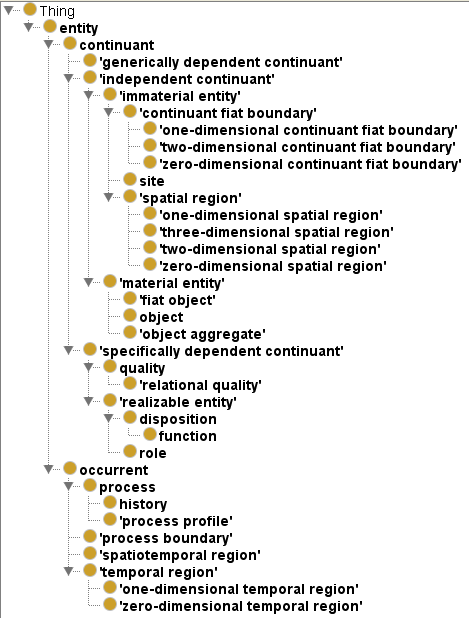
\includegraphics[scale=0.6]{author/part2/figures/chapter_kb/bfo.png}
	\label{fig:bfo}
\end{figure}

BFO --- \textit{онтология}, разработанная для поддержки совместимости данных и информационных систем, связанных с \textit{онтологиями}, содержащими более конкретные термины, относящиеся к конкретным \textit{предметным областям}.

Основная цель BFO --- поддерживать разработку таких \textit{онтологий предметной области} с тем, чтобы способствовать координации работы различных групп специалистов, добиваться непротиворечивости и предотвращать избыточность \textit{онтологий}.

Стоит отметить, что многие \textit{предметные области и онтологии}, описанные в \textit{Главе \ref{chapter_top_ontologies}~\nameref{chapter_top_ontologies}}, пересекаются с областями выделенными в BFO, но при этом BFO является более конкретной предметной онтологией. 

При этом онтология BFO не учитывает, например, ситуации и события, которые бы описывали динамику \textit{базы знаний}, что определенно необходимо для интеллектуальной системы.

Также имеет смысл рассмотреть следующие онтологии верхнего уровня:
\begin{textitemize}
	\item{\textbf{The Standard Upper Ontology} (SUMO) (см. \scncite{SUMO})}
	\item{\textbf{Descriptive Ontology for Linguistic and Cognitive Engineering} (DOLCE) (см. \scncite{DOLCE})}
\end{textitemize}

SUMO --- это онтология верхнего уровня, предназначена для использования в качестве базовой онтологии для различных компьютерных систем обработки информации. Данный проект образует большую формальную общедоступную онтологию и претендует на статус формирования стандарта для онтологий верхнего уровня, используется для исследований и приложений в области поиска, лингвистики и рассуждений. Назначение SUMO --- содействовать улучшению интероперабельности данных, извлечению и поиску информации, автоматическому выводу (доказательствам), обработке естественного языка.

Структура SUMO основана на разделении сущностей на две категории:
\begin{textitemize}
	\item абстрактные сущности;
	\item физические сущности.
\end{textitemize}

Иерархия понятий, используемых в SUMO, представлена на рисунке~\textit{\nameref{fig:sumo}}.

\begin{figure}[H]
	\caption{Рисунок. Иерархия понятий, используемых в SUMO}
	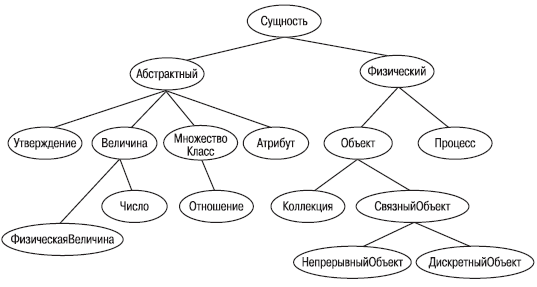
\includegraphics[scale=0.8]{author/part2/figures/chapter_kb/sumo.png}
	\label{fig:sumo}
\end{figure}

Первая категория ``Абстрактное'' включает в себя все, что имеет положение в пространстве и времени, а вторая категория включает в себя все остальное.

В свою очередь онтология DOLCE ориентирована на то, чтобы охватить онтологические категории, лежащие в основе естественного языка.

Иерархия понятий, используемых в DOLCE, представлена на рисунке~\textit{\nameref{fig:dolce}}.

\begin{figure}[H]
	\caption{Рисунок. Иерархия понятий, используемых в DOLCE}
	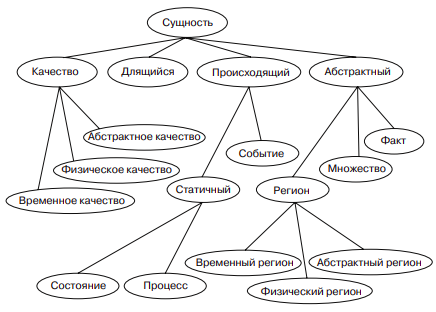
\includegraphics[scale=0.8]{author/part2/figures/chapter_kb/dolce.png}
	\label{fig:dolce}
\end{figure}

Верхний объект помечен как ``Сущность'', что указывает на то, что все экземпляры этого объекта и его подтипов являются частными по отношению к понятию ``Сущность''. У рассмотренной онтологии несомненно есть свои плюсы, такие как разделение объектов на классы во времени, однако деление классов не шаблонизировано. 

Стоит отметить, что представленный список не является окончательным. Существует более пятнадцати онтологий, претендующих на звание \textit{онтологий верхнего уровня}, целью создания которых является использование их при создании онтологий более низкого уровня.

\end{comment}

Однако попытки создать универсальную \textit{онтологию верхнего уровня}, способную обеспечить совместимость \textit{интеллектуальных компьютерных систем}, не привели к ожидаемым результатам, поскольку данные \textit{онтологии} имеют ряд ключевых недостатков:
\begin{textitemize}
	\item Каждая из представленных \textit{онтологий} является монолитной структурой, в которой нет четкой локализации на отдельные небольшие \textit{онтологии}. \\
	Главной задачей при проектировании фрагментов \textit{баз знаний} с использованием онтологического подхода является выделение \textit{онтологий} таким образом, чтобы они давали возможность относительно независимой эволюции каждого фрагмента. Структура данных \textit{онтологий верхнего уровня} представляет собой иерархию, состоящую из большого количества различных понятий. Данный вид структуризации приводит к ситуации, когда необходимость внесения изменений в одном месте обязательно повлечет за собой невозможность редактирования другой части \textit{онтологии}. В силу вышесказанного данный вид структуризации делает \textit{онтологии} неудобными для их использования при разработке различных интеллектуальных систем;
	\item Рассматриваемые \textit{онтологии верхнего уровня} не являются частью комплексной технологии.\\
	Поскольку рассматриваемые \textit{онтологии} не являются частью какой-то комплексной технологии, они не могут рассматриваться как часть \textit{библиотеки многократно используемых компонентов}. Что, в свою очередь, приводит к неудобствам в виде необходимости адаптации используемых \textit{онтологий} для каждой конкретной системы.
	\item Не существует технологий проектирования \textit{баз знаний} на основе данных \textit{онтологий верхнего уровня}.\\
	Отсутствие технологий проектирования \textit{баз знаний} затрудняет разработку интеллектуальных систем. 
\end{textitemize}

В свою очередь, \textit{Технология OSTIS} позволяет построить четкую иерархию \textit{предметных областей и онтологий}, что подразумевает легкость расширения \textit{баз знаний} и, соответственно, легкость расширения онтологий и предметных областей. Данный факт позволяет обеспечить возможность коллективной разработки \textit{баз знаний}, построенных на основе \textit{Технологии OSTIS}, а также позволяет использовать результаты, полученные в ходе работы над описанными онтологиями верхнего уровня, в ostis-системах, и собрать все лучшее от существующих ныне решений, исключая их недостатки.

\section*{Заключение к Главе \ref{chapter_kb}}
%\label{sec_sd_of_concepts}

Онтологический подход к проектированию \textit{баз знаний} \textit{интеллектуальных компьютерных систем} является ключевым в технологии проектирования \textit{баз знаний} \textit{интеллектуальных компьютерных систем} и заключается в представлении \textit{базы знаний} \textit{интеллектуальных компьютерных систем} на основе \textit{Технологии OSTIS} как иерархической структуры взаимосвязанных \textit{предметных областей} и их \textit{онтологий}, построенных на базе \textit{онтологий верхнего уровня}.

Использование данного подхода при проектировании \textit{баз знаний} \textit{интеллектуальных компьютерных систем} позволяет обеспечить совместимость интеллектуальных систем, за счет унифицированного представления \textit{знаний}. А также повысить эффективность разработки \textit{интеллектуальных компьютерных систем нового поколения}, за счет компонентного подхода к разработке \textit{баз знаний} и средств автоматизации их разработки.

%%%%%%%%%%%%%%%%%%%%%%%%% referenc.tex %%%%%%%%%%%%%%%%%%%%%%%%%%%%%%
% sample references
% %
% Use this file as a template for your own input.
%
%%%%%%%%%%%%%%%%%%%%%%%% Springer-Verlag %%%%%%%%%%%%%%%%%%%%%%%%%%
%
% BibTeX users please use
% \bibliographystyle{}
% \bibliography{}
%
\biblstarthook{In view of the parallel print and (chapter-wise) online publication of your book at \url{www.springerlink.com} it has been decided that -- as a genreral rule --  references should be sorted chapter-wise and placed at the end of the individual chapters. However, upon agreement with your contact at Springer you may list your references in a single seperate chapter at the end of your book. Deactivate the class option \texttt{sectrefs} and the \texttt{thebibliography} environment will be put out as a chapter of its own.\\\indent
References may be \textit{cited} in the text either by number (preferred) or by author/year.\footnote{Make sure that all references from the list are cited in the text. Those not cited should be moved to a separate \textit{Further Reading} section or chapter.} If the citatiion in the text is numbered, the reference list should be arranged in ascending order. If the citation in the text is author/year, the reference list should be \textit{sorted} alphabetically and if there are several works by the same author, the following order should be used:
\begin{enumerate}
\item all works by the author alone, ordered chronologically by year of publication
\item all works by the author with a coauthor, ordered alphabetically by coauthor
\item all works by the author with several coauthors, ordered chronologically by year of publication.
\end{enumerate}
The \textit{styling} of references\footnote{Always use the standard abbreviation of a journal's name according to the ISSN \textit{List of Title Word Abbreviations}, see \url{http://www.issn.org/en/node/344}} depends on the subject of your book:
\begin{itemize}
\item The \textit{two} recommended styles for references in books on \textit{mathematical, physical, statistical and computer sciences} are depicted in ~\cite{science-contrib, science-online, science-mono, science-journal, science-DOI} and ~\cite{phys-online, phys-mono, phys-journal, phys-DOI, phys-contrib}.
\item Examples of the most commonly used reference style in books on \textit{Psychology, Social Sciences} are~\cite{psysoc-mono, psysoc-online,psysoc-journal, psysoc-contrib, psysoc-DOI}.
\item Examples for references in books on \textit{Humanities, Linguistics, Philosophy} are~\cite{humlinphil-journal, humlinphil-contrib, humlinphil-mono, humlinphil-online, humlinphil-DOI}.
\item Examples of the basic Springer style used in publications on a wide range of subjects such as \textit{Computer Science, Economics, Engineering, Geosciences, Life Sciences, Medicine, Biomedicine} are ~\cite{basic-contrib, basic-online, basic-journal, basic-DOI, basic-mono}. 
\end{itemize}
}

\begin{thebibliography}{99.}%
% and use \bibitem to create references.
%
% Use the following syntax and markup for your references if 
% the subject of your book is from the field 
% "Mathematics, Physics, Statistics, Computer Science"
%
% Contribution 
\bibitem{science-contrib} Broy, M.: Software engineering --- from auxiliary to key technologies. In: Broy, M., Dener, E. (eds.) Software Pioneers, pp. 10-13. Springer, Heidelberg (2002)
%
% Online Document
\bibitem{science-online} Dod, J.: Effective substances. In: The Dictionary of Substances and Their Effects. Royal Society of Chemistry (1999) Available via DIALOG. \\
\url{http://www.rsc.org/dose/title of subordinate document. Cited 15 Jan 1999}
%
% Monograph
\bibitem{science-mono} Geddes, K.O., Czapor, S.R., Labahn, G.: Algorithms for Computer Algebra. Kluwer, Boston (1992) 
%
% Journal article
\bibitem{science-journal} Hamburger, C.: Quasimonotonicity, regularity and duality for nonlinear systems of partial differential equations. Ann. Mat. Pura. Appl. \textbf{169}, 321--354 (1995)
%
% Journal article by DOI
\bibitem{science-DOI} Slifka, M.K., Whitton, J.L.: Clinical implications of dysregulated cytokine production. J. Mol. Med. (2000) doi: 10.1007/s001090000086 
%
\bigskip

% Use the following (APS) syntax and markup for your references if 
% the subject of your book is from the field 
% "Mathematics, Physics, Statistics, Computer Science"
%
% Online Document
\bibitem{phys-online} J. Dod, in \textit{The Dictionary of Substances and Their Effects}, Royal Society of Chemistry. (Available via DIALOG, 1999), 
\url{http://www.rsc.org/dose/title of subordinate document. Cited 15 Jan 1999}
%
% Monograph
\bibitem{phys-mono} H. Ibach, H. L\"uth, \textit{Solid-State Physics}, 2nd edn. (Springer, New York, 1996), pp. 45-56 
%
% Journal article
\bibitem{phys-journal} S. Preuss, A. Demchuk Jr., M. Stuke, Appl. Phys. A \textbf{61}
%
% Journal article by DOI
\bibitem{phys-DOI} M.K. Slifka, J.L. Whitton, J. Mol. Med., doi: 10.1007/s001090000086
%
% Contribution 
\bibitem{phys-contrib} S.E. Smith, in \textit{Neuromuscular Junction}, ed. by E. Zaimis. Handbook of Experimental Pharmacology, vol 42 (Springer, Heidelberg, 1976), p. 593
%
\bigskip
%
% Use the following syntax and markup for your references if 
% the subject of your book is from the field 
% "Psychology, Social Sciences"
%
%
% Monograph
\bibitem{psysoc-mono} Calfee, R.~C., \& Valencia, R.~R. (1991). \textit{APA guide to preparing manuscripts for journal publication.} Washington, DC: American Psychological Association.
%
% Online Document
\bibitem{psysoc-online} Dod, J. (1999). Effective substances. In: The dictionary of substances and their effects. Royal Society of Chemistry. Available via DIALOG. \\
\url{http://www.rsc.org/dose/Effective substances.} Cited 15 Jan 1999.
%
% Journal article
\bibitem{psysoc-journal} Harris, M., Karper, E., Stacks, G., Hoffman, D., DeNiro, R., Cruz, P., et al. (2001). Writing labs and the Hollywood connection. \textit{J Film} Writing, 44(3), 213--245.
%
% Contribution 
\bibitem{psysoc-contrib} O'Neil, J.~M., \& Egan, J. (1992). Men's and women's gender role journeys: Metaphor for healing, transition, and transformation. In B.~R. Wainrig (Ed.), \textit{Gender issues across the life cycle} (pp. 107--123). New York: Springer.
%
% Journal article by DOI
\bibitem{psysoc-DOI}Kreger, M., Brindis, C.D., Manuel, D.M., Sassoubre, L. (2007). Lessons learned in systems change initiatives: benchmarks and indicators. \textit{American Journal of Community Psychology}, doi: 10.1007/s10464-007-9108-14.
%
%
% Use the following syntax and markup for your references if 
% the subject of your book is from the field 
% "Humanities, Linguistics, Philosophy"
%
\bigskip
%
% Journal article
\bibitem{humlinphil-journal} Alber John, Daniel C. O'Connell, and Sabine Kowal. 2002. Personal perspective in TV interviews. \textit{Pragmatics} 12:257--271
%
% Contribution 
\bibitem{humlinphil-contrib} Cameron, Deborah. 1997. Theoretical debates in feminist linguistics: Questions of sex and gender. In \textit{Gender and discourse}, ed. Ruth Wodak, 99--119. London: Sage Publications.
%
% Monograph
\bibitem{humlinphil-mono} Cameron, Deborah. 1985. \textit{Feminism and linguistic theory.} New York: St. Martin's Press.
%
% Online Document
\bibitem{humlinphil-online} Dod, Jake. 1999. Effective substances. In: The dictionary of substances and their effects. Royal Society of Chemistry. Available via DIALOG. \\
http://www.rsc.org/dose/title of subordinate document. Cited 15 Jan 1999
%
% Journal article by DOI
\bibitem{humlinphil-DOI} Suleiman, Camelia, Daniel C. O'Connell, and Sabine Kowal. 2002. `If you and I, if we, in this later day, lose that sacred fire...': Perspective in political interviews. \textit{Journal of Psycholinguistic Research}. doi: 10.1023/A:1015592129296.
%
%
%
\bigskip
%
%
% Use the following syntax and markup for your references if 
% the subject of your book is from the field 
% "Computer Science, Economics, Engineering, Geosciences, Life Sciences"
%
%
% Contribution 
\bibitem{basic-contrib} Brown B, Aaron M (2001) The politics of nature. In: Smith J (ed) The rise of modern genomics, 3rd edn. Wiley, New York 
%
% Online Document
\bibitem{basic-online} Dod J (1999) Effective Substances. In: The dictionary of substances and their effects. Royal Society of Chemistry. Available via DIALOG. \\
\url{http://www.rsc.org/dose/title of subordinate document. Cited 15 Jan 1999}
%
% Journal article by DOI
\bibitem{basic-DOI} Slifka MK, Whitton JL (2000) Clinical implications of dysregulated cytokine production. J Mol Med, doi: 10.1007/s001090000086
%
% Journal article
\bibitem{basic-journal} Smith J, Jones M Jr, Houghton L et al (1999) Future of health insurance. N Engl J Med 965:325--329
%
% Monograph
\bibitem{basic-mono} South J, Blass B (2001) The future of modern genomics. Blackwell, London 
%
\end{thebibliography}
